\documentclass{beamer}

\usepackage[utf8]{inputenc}
\usepackage{subfigure}
\usepackage{caption}

\title{Multimodal Corpora}
\subtitle{A brief summary with three examples}
\author{Tuan Pham Minh, Nils Harder, Tilman Krokotsch}
\date{January 17, 2017}

\begin{document}

	\beamertemplatenavigationsymbolsempty
	\setbeamercolor{title}{fg=black}
	\setbeamercolor{frametitle}{fg=black}
	\setbeamercolor{local structure}{fg=black}
	
	\setcounter{tocdepth}{1}

	\maketitle
	
	\begin{frame}
		\tableofcontents
	\end{frame}
	
	\section{BAS SmartKom Corpus} 	
	\subsection{General Information}
			\begin{frame}{The BAS SmartKom Corpus}{General Information}			
				\begin{itemize}
					\item released in 2001
					\cite{basSKP}
					\item extended and finalized in 2003
					\item modalities:
					\begin{itemize}
						\item 10 Audio streams
						\item 4 Video streams
						\item annotations including gestures and emotions
					\end{itemize}
					\item part of the SmartKom projectu
				\end{itemize}											
			\end{frame}		
			\begin{frame}{The BAS SmartKom Corpus}{General Information}			
				\begin{itemize}
					\item collaborative work:
					\begin{itemize}
						\item Universities
						\begin{itemize}
							\item Munich
							\item Erlangen
							\item Stuttgart
						\end{itemize}
						\item Industrial partners
						\begin{itemize}
							\item Daimler/Chrysler
							\item DFKI
							\item European Media Lab
							\item Philips
							\item Media Interface
							\item Siemens
							\item SONY
						\end{itemize}
					\end{itemize}
				\end{itemize}											
			\end{frame}		
			
		\subsection{Motivation}
			\begin{frame}{The BAS SmartKom Corpus}{Motivation}			
				\begin{itemize}
					\item exploring natural multi-modal Computer-User-Interfaces
					\item focus on laypeople and unsupervised usage
					\item large variance in tasks and environments
				\end{itemize}											
			\end{frame}		
				
		\subsection{Recording Scenario}
			\begin{frame}{The BAS SmartKom Corpus}{Recording Scenario}																\begin{figure}
					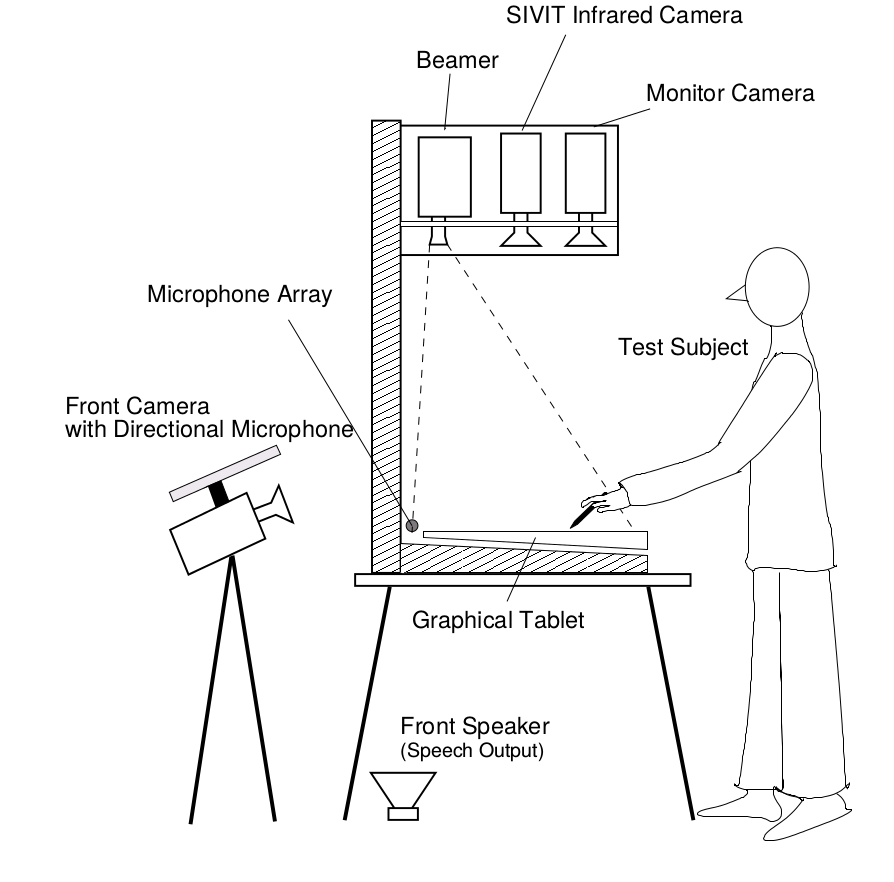
\includegraphics[width=0.7\textwidth]{images/BAS/setup}
					\caption{The 'Public' Recording Setup}
					\vspace*{-10pt}
					\caption*{Source: \cite{basSKP}}
				\end{figure}
			\end{frame}
		
		\subsection{Recorded Data}
			\begin{frame}{The BAS SmartKom Corpus}{Primary Data}										
				\begin{itemize}
					\item Video of face, frontal and fixed position
					\item Video of the upper body, from the left, fixed
					\item Infrared Video of projected Interface for Hand tracking
					\item 10 Audio channels
					\begin{itemize}
						\item 4 element microphone array
						\item directed microphone
						\item headset and/or lapel microphone
						\item stereo background noise 
						\item system output
					\end{itemize}
					\item Graphical System output, low framerate
					\item Combined Stream of all 4 video streams
					\item Coordinates of finger tip or pencil position		
				\end{itemize}
			\end{frame}
			
		\begin{frame}{The BAS SmartKom Corpus}{Secondary Data}
			\begin{itemize}
				\item Transliteration of audio channel 
				\item Turn segmentation
				\item Segmentation and labeling of gestures in two dimensions
				\item Segmentation and labeling of user state
				\begin{itemize}
					\item using facial and speech information
					\item using only facial information 
				\end{itemize}
				\item Segmentation and labeling of prosodic features to recognize emotions
			\end{itemize}
		\end{frame}
		\begin{frame}{The BAS SmartKom Corpus}{Example Data}
		\begin{figure}
			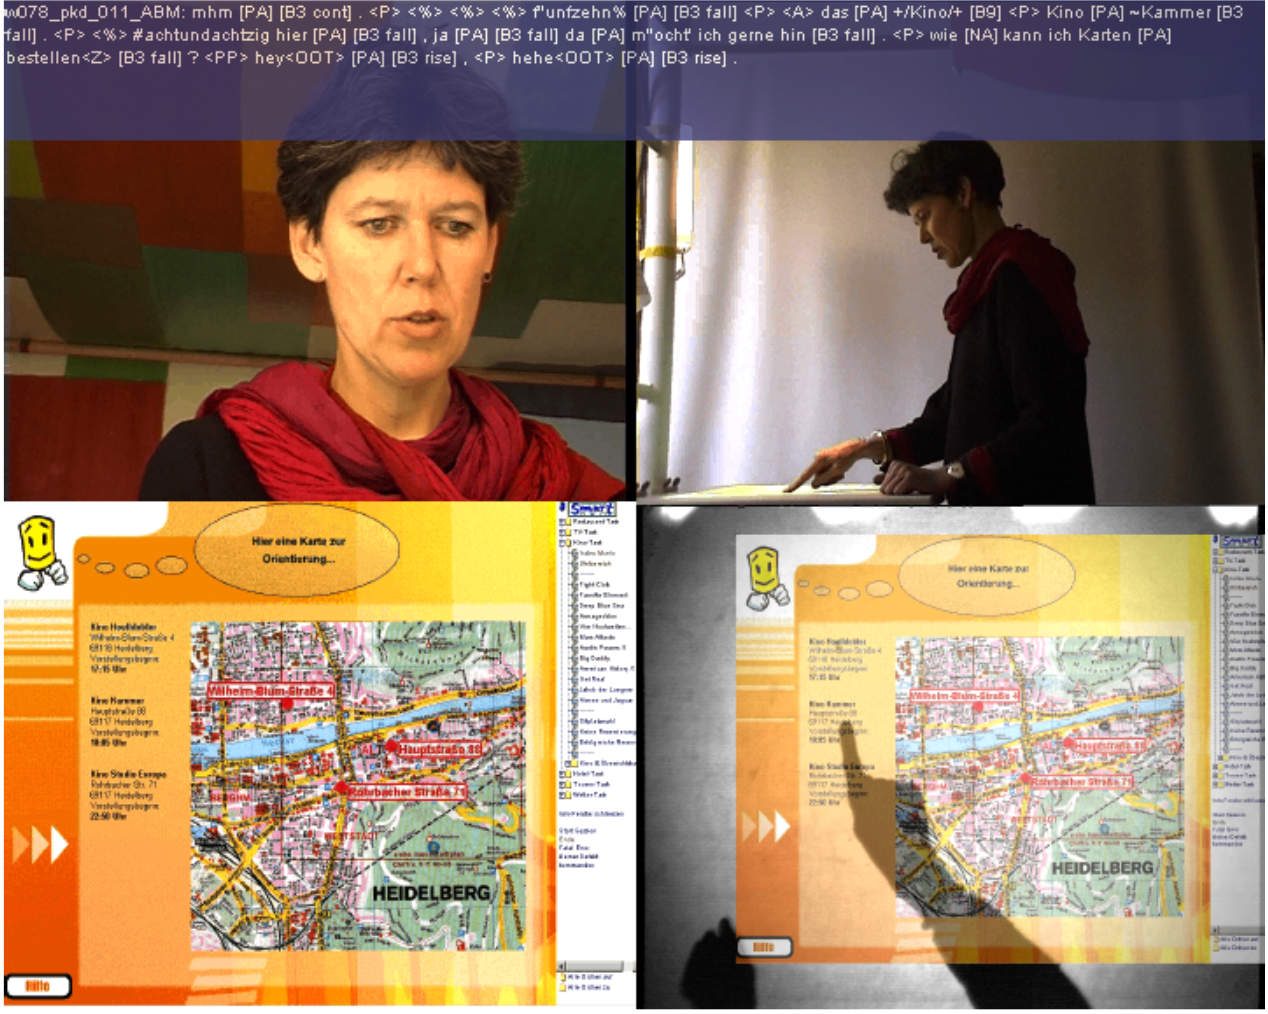
\includegraphics[width=0.8\textwidth]{images/BAS/stream}
			\caption{Unified QuickTime stream}
			\vspace*{-10pt}
			\caption*{Source: \cite{basSKP}}	
			\end{figure}		
		\end{frame}
		
		\subsection{Application}
			\begin{frame}{The BAS SmartKom Corpus}{Application}
				\begin{itemize}
					\item audio-only subset used for emotion research (SKAUDIO)
					\item research into the properties of symmetric multi-modal Interfaces\cite{wahlster2003towards}
				\end{itemize}
			\end{frame}	
	
	\section{The CALLAS Expressivity Corpus}			
		\subsection{General Information}
				\begin{frame}{The CALLAS Expressivity Corpus}{Motivation}			
					\begin{itemize}
						\item not yet released
						\item first introduced in 2010 \cite{2010MultimodalCorpusForGestureExpressivity}
						\item second publication with a more detailed description and first results in 2013 \cite{Caridakis2013}
						\item modalities:
						\begin{itemize}
							\item audio
							\item video
							\item gestures
						\end{itemize}
						\item part of the Conveying Affectiveness in Leading edge Living Adaptive
	Systems (Callas) project
					\end{itemize}											
				\end{frame}		
				\begin{frame}{The CALLAS Expressivity Corpus}{Motivation}			
					\begin{itemize}
						\item collaborative work:
						\begin{itemize}
							\item National Technical University of Athens
								\begin{itemize}
									\item G. Caridakis
									\item A. Raouzaiou
									\item K. Karpouzis
								\end{itemize}
							\item the Augsburg University
								\begin{itemize}
									\item J. Wagner
									\item F. Lingenfelser
									\item E. Andre
								\end{itemize}
							\item Humanware S.r.l.
								\begin{itemize}
									\item Z. Curto
								\end{itemize}
						\end{itemize}
					\end{itemize}											
				\end{frame}		
				
			\subsection{Motivation}
				\begin{frame}{The CALLAS Expressivity Corpus}{Motivation}			
					\begin{itemize}
						\item capturing cross-cultural differences in gestural emotion expression
						\item creating a more realistic corpus with a high variance in data
					\end{itemize}											
				\end{frame}		
					
			\subsection{Recording Scenario}
				\begin{frame}{The CALLAS Expressivity Corpus}{Recording Scenario}																\begin{figure}
						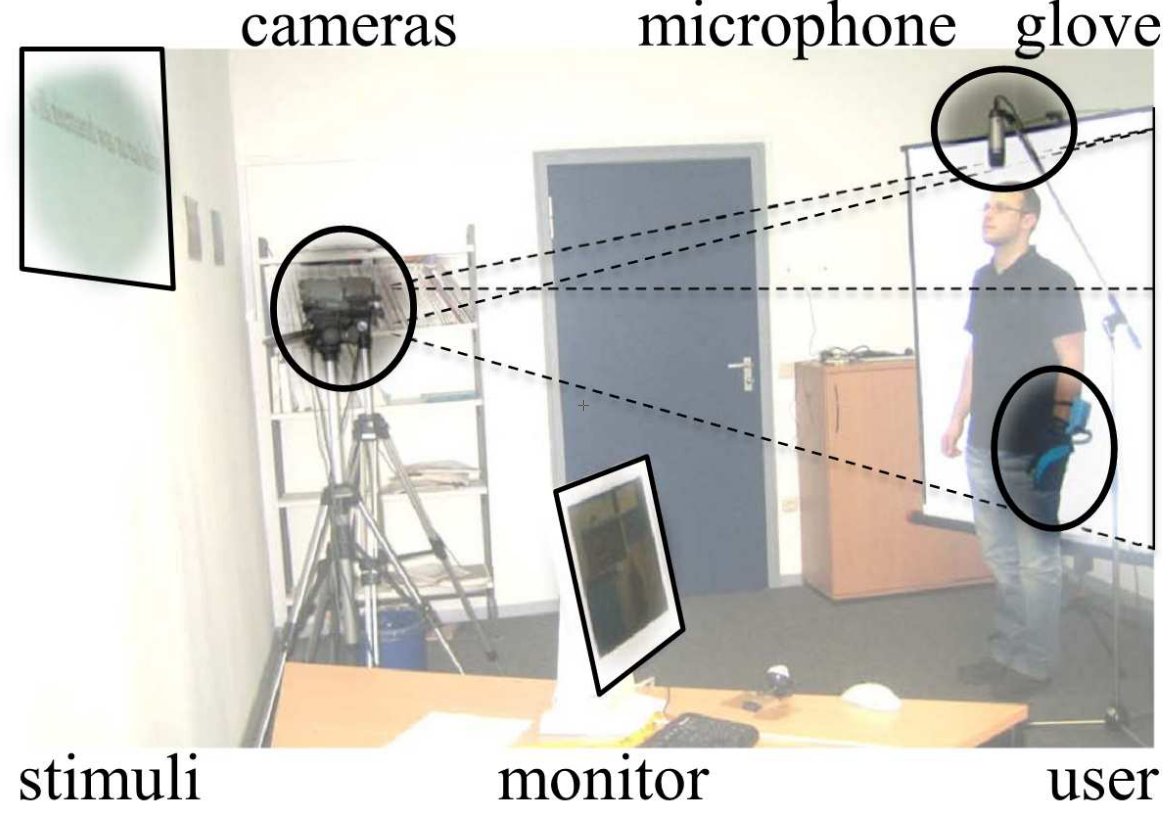
\includegraphics[width=0.8\textwidth]{images/Callas/experimentSetup}
						\caption{Experiment setup}
						\vspace*{-10pt}
						\caption*{Source: \cite{2010MultimodalCorpusForGestureExpressivity}}
					\end{figure}
				\end{frame}
			
			\subsection{Recorded Data}
				\begin{frame}{The CALLAS Expressivity Corpus}{Recorded Data}										
					\begin{itemize}
						\item Modalities:
						\begin{itemize}
							\item Audio:
							 \begin{itemize}
							 	\item Mono
							 	\item 16 kHz sampling rate
							 \end{itemize}
							 \item Video
							 \begin{itemize}
							 	\item 2 video streams
							 	\item 720 x 576px
							 	\item 25 fps
							 	\item 24 bit colour depth
							 \end{itemize}
							 \item Gesture
							 \begin{itemize}
							 	\item bare hands: position of hands
							 	\item Wiimote: accelerometer data
							 	\item data glove:angles between finger joints
							 \end{itemize}
						\end{itemize}
					\end{itemize}
				\end{frame}
			\subsection{Application}
				\begin{frame}{The CALLAS Expressivity Corpus}{Application}
					\begin{itemize}
						\item study cross-cultural differences
						\item compare approaches to combine different modalities
					\end{itemize}
				\end{frame}	
		
	\section{The Bielefeld Speech and Gesture Alignment Corpus}
		\subsection{Recording Scenario}
			\begin{frame}{The Bielefeld Speech and Gesture Alignment Corpus}{Recording Scenario}
				\begin{figure}
					\subfigure{
						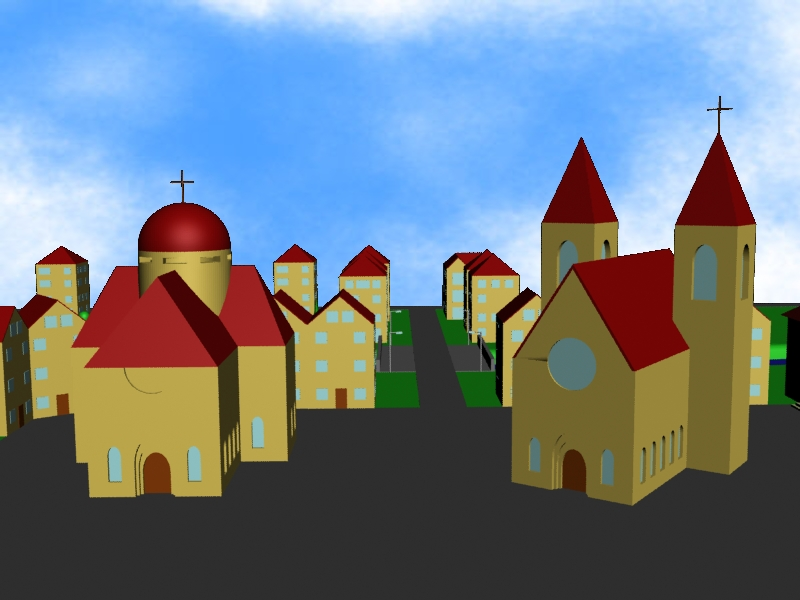
\includegraphics[width=0.48\textwidth]{Scenario}
					}
					\subfigure{
						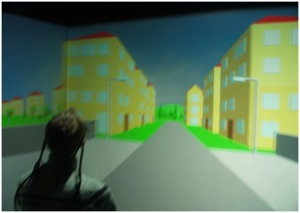
\includegraphics[width=0.48\textwidth]{Scenario_2}
					}
				\end{figure}
			\end{frame}
		
		\subsection{Recorded Data}
			
				\begin{frame}{The Bielefeld Speech and Gesture Alignment Corpus}{Primary Data}
					\begin{figure}
						\subfigure{
								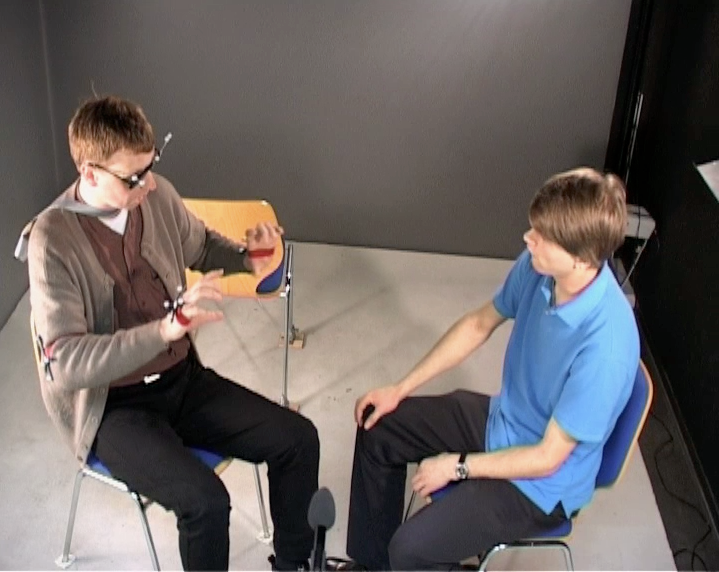
\includegraphics[width=0.4\textwidth]{Primary_1}
						}
						\subtable{
							\resizebox{0.5\textwidth}{!}{%
							\begin{tabular}{|l|c|}
								\hline 
								\textbf{Specification} & \textbf{Value} \\ 
								\hline 
								Number of dialogs & 25 \\ 
								\hline 
								Video time & 280 minutes \\ 
								\hline 
								Video specification & 720x576, 25fps  \\ 
								\hline 
								Video codec & H.264  \\ 
								\hline 
								Video feeds & 3 \\ 
								\hline 
								Audio feeds & 1 \\ 
								\hline
							\end{tabular} 
							}
						}
					\end{figure}
				\end{frame}
			
				\begin{frame}{The Bielefeld Speech and Gesture Alignment Corpus}{Secondary Data}
					\begin{figure}
					\subfigure{
						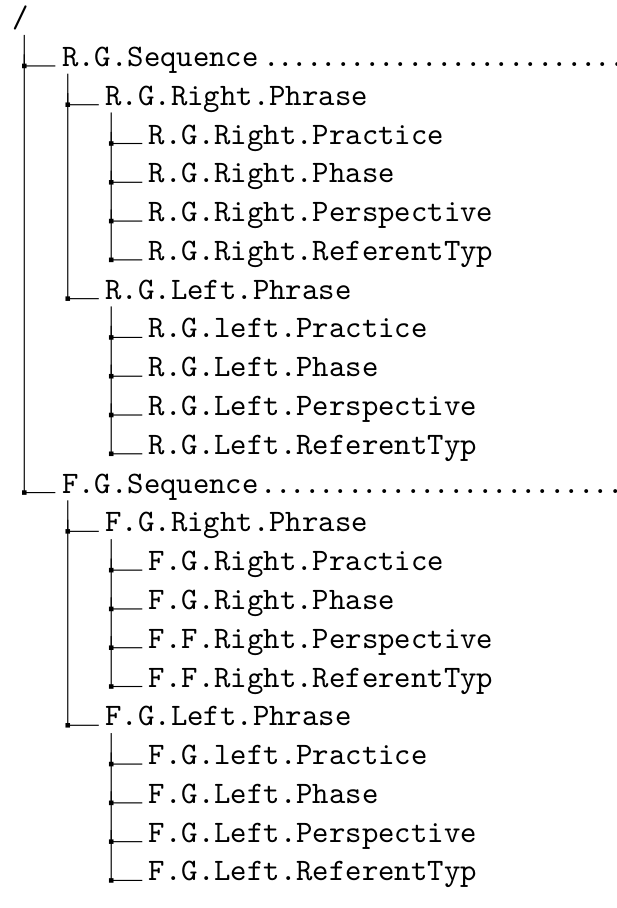
\includegraphics[width=0.45\textwidth]{Annotation_Scheme}
					}
					\subfigure{
						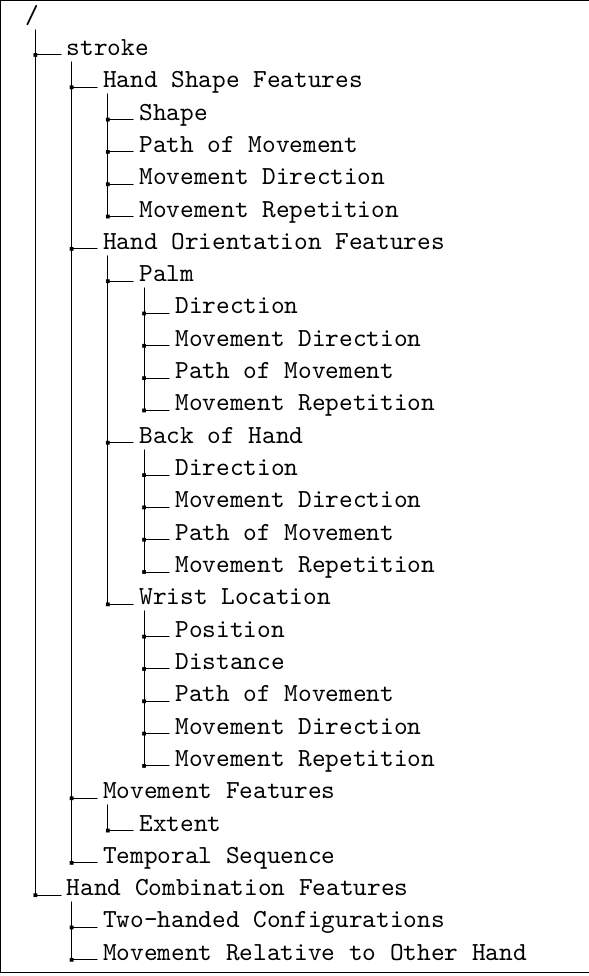
\includegraphics[width=0.45\textwidth]{Annotation_Scheme_2}
					}
				\end{figure}
				\end{frame}
			
				\begin{frame}{The Bielefeld Speech and Gesture Alignment Corpus}{Secondary Data}
					\begin{table}
						\center
						\begin{tabular}{|l|c|}
							\hline
							\textbf{Specification} & \textbf{Value} \\ 
							\hline 
							Words & 39,435 \\ 
							\hline 
							Iconic/Deictic gestures & 4961 \\ 
							\hline 
							Discourse gestures & approx. 1000 \\ 
							\hline 
						\end{tabular}
					\end{table}
				\end{frame}
		
		\subsection{Application}
			\begin{frame}{The Bielefeld Speech and Gesture Alignment Corpus}{Application}
				\center
						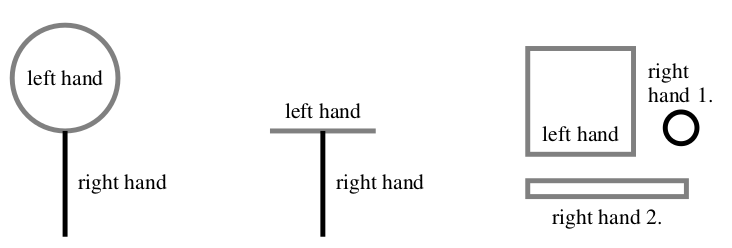
\includegraphics[width=0.7\textwidth]{Types}
						\vspace*{1cm}
						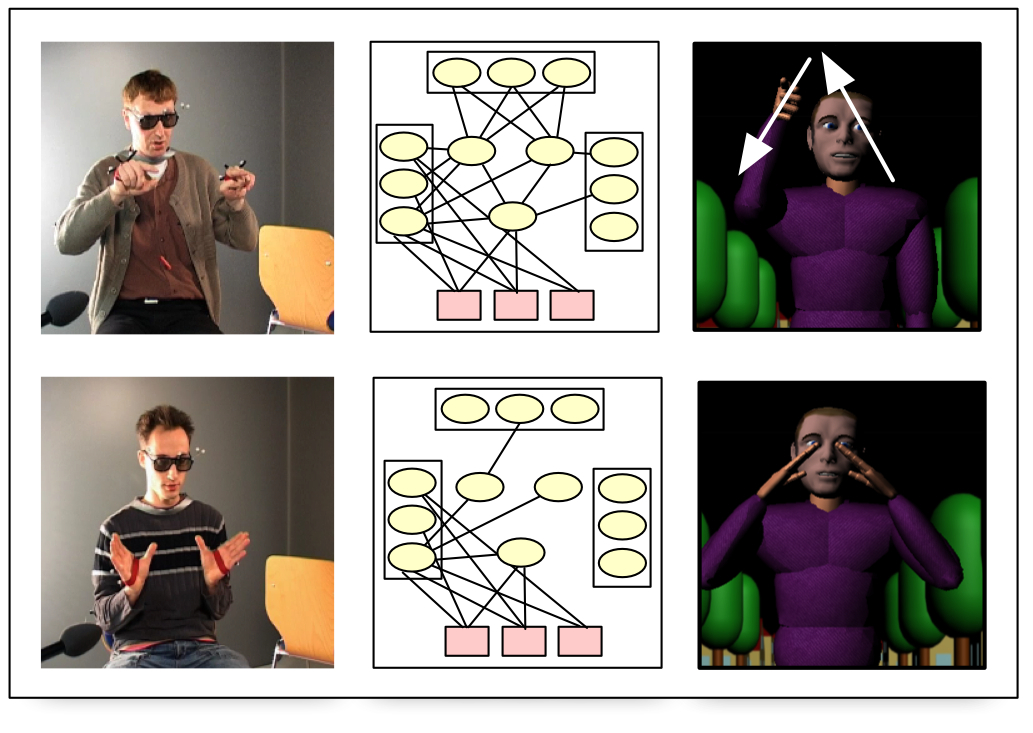
\includegraphics[width=0.6\textwidth]{Bayes}
			\end{frame}	
	
	\section{Sources}
		\begin{frame}[allowframebreaks]{Sources}
			\bibliographystyle{IEEEtran}
			\nocite{Bielefeld2010}
			\nocite{Bielefeld2013}
			\nocite{Bergmann2014}
			\nocite{BAS2014}

  			\small\bibliography{../thebib}
		\end{frame}
	
\end{document}